\documentclass[springer.tex]{subfiles}
\graphicspath{ {./figures/} }

\begin{document}
\chapter{Imperative programming stuff}
\section{Variables}
\label{sec:mutableValues}
Identifiers may be mutable, which means that the it may be rebound to a new value. Mutable identifiers are specified using the \idx[mutable@\lstinline{mutable}]{\keyword{mutable}} keyword with the following syntax:
%
\begin{verbatimwrite}{\ebnf/variables.ebnf}
let mutable <*ident*> = <*expr*> [*in <*expr*>*]
\end{verbatimwrite}
\syntax{\ebnf/variables.ebnf}{Syntax for defining mutable values with an initial value.}
%
Changing the value of an identifier is called \idx{assignment} and is done using the \idx[{<-}@\lstinline{<-}]{\lexeme{<-}} lexeme. Assignments have the following syntax:\jon{Discussion on heap and stack should be added here.}
%
\begin{verbatimwrite}{\ebnf/assignment.ebnf}
<*ident*> <- <*ident*>
\end{verbatimwrite}
\syntax{\ebnf/assignment.ebnf}{Value reassignment for mutable variables.}
%
\idx[mutable value]{Mutable values} is synonymous with the term \idx{variable}. A variable is an area in the computer's working memory associated with an identifier and a type, and this area may be read from and written to during program execution, see \Cref{mutableAssignReassingShort} for an example.
%
\fs{mutableAssignReassingShort}{A variable is defined and later reassigned a new value.}
%\fs{mutableAssignReassing}{}
%
Here, an area in memory was denoted \lstinline{x}, initially assigned the integer value 5, hence the type was inferred to be \lstinline|int|.  Later, this value of \lstinline{x} was replaced with another integer using the \lexeme{<-} lexeme. The \lexeme{<-} lexeme is used to distinguish the assignment from the comparison operator. For example, the statement \lstinline{a = 3} in \Cref{mutableEqual} is not an assignment but a comparison which is evaluated to be false. 
%
\fsOutput{mutableEqual}{It is a common error to mistake \lexeme{=} and \lexeme{<-} lexemes for mutable variables.}
% \begin{lstlisting}[language=fsharp,caption={fsharpi, example of changing the content of a variable.}]
% > let mutable a = 0
% - a = 3;;
%
% val mutable a : int = 0
% val it : bool = false
% \end{lstlisting}
%
However, it is important to note that when the variable is initially defined, then the '\lexeme{=}' operator must be used, while later reassignments must use the \lexeme{<-} expression.

Assignment type mismatches will result in an error, as demonstrated in \Cref{mutableAssignReassingTypeError}. 
%
\fs{mutableAssignReassingTypeError}{Assignment type mismatching causes a compile-time error.}
%
I.e., once the type of an identifier has been declared or inferred, it cannot be changed.

A typical variable is a counter of type integer, and a typical use of counters is to increment them, see \Cref{mutableAssignIncrement} for an example.
%
\fs{mutableAssignIncrement}{Variable increment is a common use of variables.}
%
Using variables in expressions, as opposed to the left-hand-side of an assignment operation, reads the value of the variable. Thus, when using a variable as the return value of a function, then the value is copied from the local scope of the function to the scope from which it is called. This is demonstrated in \Cref{mutableAssignReturnVariable}.
%
\fsOutput{mutableAssignReturnVariable}{Returning a mutable variable returns its value.}
%
In the example we see that the type is a value, and not mutable. 

Variables implement dynamic scope, that is, the value of an identifier depends on \emph{when} it is used. This is in contrast to lexical scope, where the value of an identifier depends on \emph{where} it is defined. As an example, consider the script in \Cref{lexicalScopeNFunction} which defines a function using lexical scope and returns the number \lstinline!6.0!, however, if \lstinline!a! is made \lstinline!mutable!, then the behavior is different, as shown in \Cref{dynamicScopeNFunction}.
%
\fs{dynamicScopeNFunction}{Mutual variables implement dynamic scope rules. Compare with \Cref{lexicalScopeNFunction}.}
%
Here, the response is \lstinline!8.0!, since the value of \lstinline!a! changed before the function \lstinline!f! was called.

\section{Reference Cells}
\label{sec:referenceCells}
%F\# has a variation of mutable variables called \idx{reference cells}. Reference cells have built-in function \idx[ref@\lstinline{ref}]{\lstinline{ref}} and operators \idx[{!}@\lstinline{!}]{\lexeme{!}} and \idx[{:=}@\lstinline{:=}]{\lexeme{:=}}, where \lstinline{ref} creates a reference variable, and the '\lexeme{!}' and the '\lexeme{:=}' operators reads and writes its value. An example of using reference cells is given in \Cref{refCell}.
F\# has a variation of mutable variables called \idx{reference cells}. Reference cells have the built-in function \idx[ref@\lstinline{ref}]{\lstinline{ref}} and the operators \lexeme{!} and \idx[{:=}@\lstinline{:=}]{\lexeme{:=}}, where \lstinline{ref} creates a reference variable, and the '\lexeme{!}' and the '\lexeme{:=}' operators respectively reads and writes its value. An example of using reference cells is given in \Cref{refCell}.
%
\fs{refCell}{Reference cells are variants of mutable variables.}
%
Reference cells are different from mutable variables, since their content is allocated on \idx{The Heap}. The Heap is a global data storage that is not destroyed when a function returns, which is in contrast to the \idx{call stack}, also known as \idx{The Stack}. The Stack maintains all the local data for a specific instance of a function call, see \Cref{sec:callStack} for more details. As a consequence, when a reference cell is returned from a function, then it is the reference to the location on The Heap, which is returned as a value. Since this points outside the local data area of the function, this location is still valid after the function returns, and the variable stored there is accessible to the caller. This is illustrated in \Cref{fig:returningRefCells}
%
\begin{figure}
  \centering
  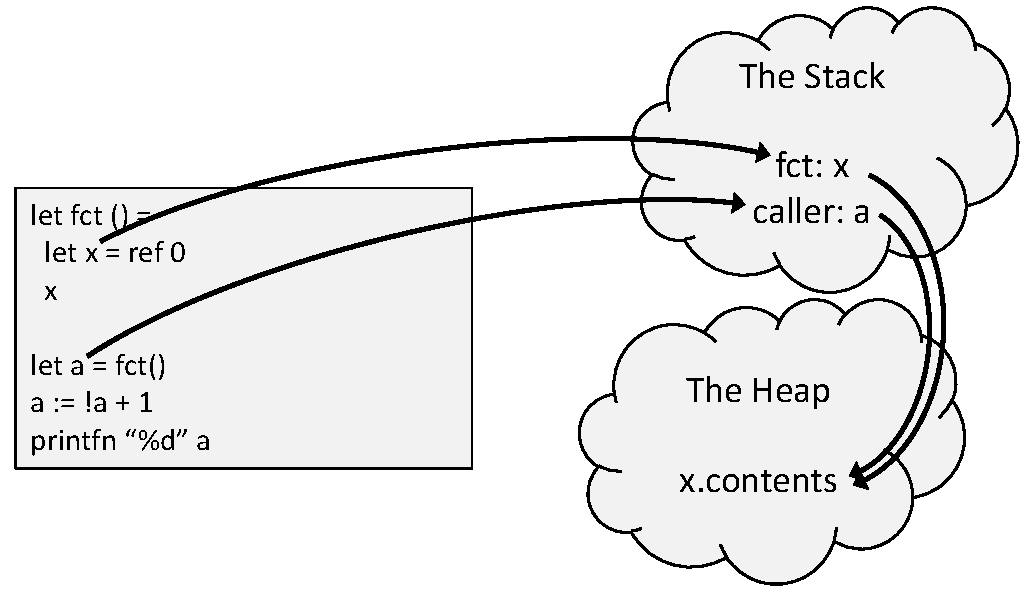
\includegraphics[width=0.6\textwidth]{ReferenceCells}
  \caption{A reference cell is a pointer to The Heap, and the content is not destroyed when its reference falls out of scope.}
  \label{fig:returningRefCells}
\end{figure}
%

Reference cells may cause \idx[side-effect]{side-effects}, where variable changes are performed across independent scopes. Some side-effects are useful, e.g., the \lstinline{printf} family changes the content of the screen, and the screen is outside the scope of the caller.  Another example of a useful side-effect is a counter shown in \Cref{refEncapsulation}.
%
\fs{refEncapsulation}{An increment function with a local state using a reference cell.}
%
Here \lstinline{incr} is an anonymous function with an internal state \lstinline{counter}. At first glance, it may be surprising that \lstinline{incr ()} does not return the value \lstinline{1} at every call. The reason is that the value of the \lstinline{incr} is the closure of the anonymous function \lstinline{fun () -> counter := ...}, which is 
\begin{equation}
  \text{\lstinline{incr}}: \left(\text{args}, \text{exp}, \text{env}\right)  = \big((), \left(\begin{subarray}{l}\displaystyle\text{\lstinline{counter := !counter + 1}}\\\displaystyle\text{\lstinline{!counter}}\end{subarray}\right), (\text{\lstinline{counter}}\rightarrow\text{\lstinline{ref 0}})\big).
\end{equation}
Thus, \lstinline{counter} is only initiated once at the initial binding, while every call of \lstinline{incr ()} updates its value on The Heap. Such a programming structure is called \idx{encapsulation}, since the \lstinline{counter} state has been encapsulated in the anonymous function, and the only way to access it is by calling the same anonymous function. In general, it is advisable to \advice{use encapsulation to hide implementation details irrelevant to the user of the code.}

The \lstinline{incr} example in \Cref{refEncapsulation} is an example of a useful side-effect. An example to be avoided is shown in \Cref{refSideEffect}.
%
\fs{refSideEffect}{Intertwining independent scopes is typically a bad idea.}
%
In the example, the function \lstinline{updateFactor} changes a variable in the scope of the function \lstinline{multiplyWithFactor}. The code style is prone to errors, since the computations are not local at the place of writing, i.e., in \lstinline{multiplyWithFactor}, and if \lstinline{updateFactor} were defined in a library, then the source code may not be available. Better style of programming is shown in \Cref{refWithoutSideEffect}.
%
\fs{refWithoutSideEffect}{A solution similar to \Cref{refSideEffect} without side-effects.}
%
Here, there can be no doubt in \lstinline{multiplyWithFactor} that the value of \lstinline{a} is changing. Side-effects do have their use, but should, in general, be avoided at almost all costs, and it is advised to \advice{minimize the use of side effects}.

Reference cells give rise to an effect called \idx{aliasing}, where two or more identifiers refer to the same data, as illustrated in \Cref{refCellAliasing}.
%
\fs{refCellAliasing}{Aliasing can cause surprising results and should be avoided.}
%
Here, \lstinline!a! is defined as a reference cell, and by defining \lstinline!b! to be equal to \lstinline!a!, we have created an alias. This can be very confusing since as the example shows, changing the value of \lstinline!b! causes \lstinline!a! to change as well. Aliasing is a variant of side-effects, and \advice{aliasing should be avoided at all costs}.

Since F\# version 4.0, the compiler has automatically converted mutable variables to reference cells, where needed.  E.g., \Cref{refEncapsulation} can be rewritten using a mutable variable, as shown in \Cref{mutableEncapsulation}.
% 
\fs{mutableEncapsulation}{Local mutable content can be indirectly accessed outside its scope.}
% 
Reference cells are preferred over mutable variables for encapsulation, in order to avoid confusion.

\end{document}
